\section{Architecture}
\label{sec:arch}

\begin{figure}
    \centering
    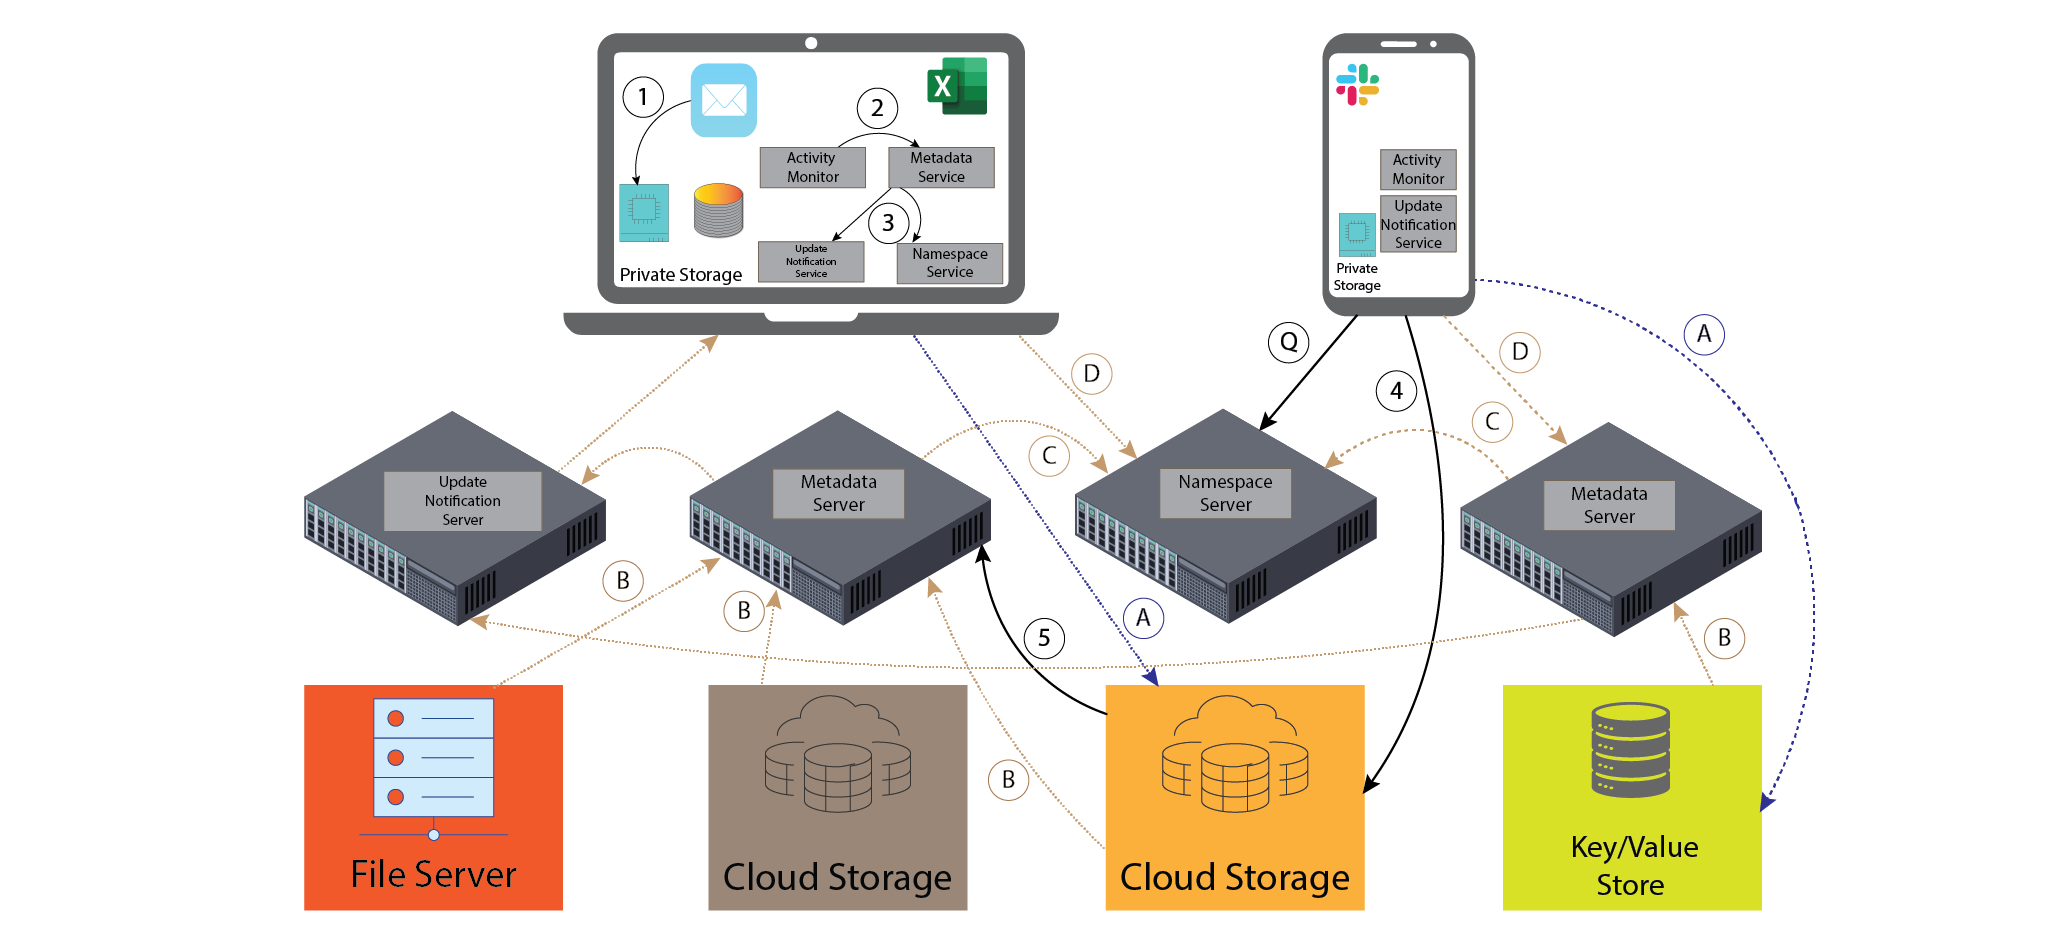
\includegraphics[width=0.45\textwidth]{figures/naming3.png}
    \caption{\system Architecture (\S \ref{sec:arch})}
    \label{fig:arch}
\end{figure}

%\reto{Using meta-data service that must inter-operate (federated meta data) and relationships are not first-class citizen, cannot glue the meta-data service together with naming services to enable the things we want to do. }
%\reto{the storage location is independent on the notion of related files: meta-data service treats relationships as first-class citizens. }
%\reto{get the attributes out of the silos --> currently: this is done manually}

\reto{No application must change, they can change. Existing browser should be able to use it, can use it to create new namespaces}

\system is a family of services that enable sophisticated search and naming capabilities.
The key features that differentiate \system from prior work are: 
\textit{1)} incorporating object relationships as first class meta-data,
\textit{2)} federating meta-data services,
\textit{3)} recording activity context,
\textit{4)} integrating storage from multiple silos, and
\textit{5)} enabling customizable naming services.
Data continues to reside in existing and to-be-developed storage silos.
\system interacts with these silos, collects and captures metadata, and 
provides a federated network of metadata and naming services to
meet the needs of the use cases in \S \ref{sec:use-cases}.


\subsection{\system Services}

Figure \ref{fig:arch} illustrates the \system architecture. There are four main components:

\noindent\textbf{1) Metadata servers (MS)}
are responsible for storing attributes and provide a superset of capabilities found in existing metadata services~\cite{federatedMetaData,smartstore}. Users can register an MS with activity monitors or attribute services to retrieve update notifications on the storage objects and activities. Thus, there can be multiple sources of attributes including the user itself. Metadata servers may retain the full or partial history of attribute updates, or just keep the last value. 

% Users register metadata servers (MS) with storage silos (sparkly arrow A) providing credentials that the silo uses to transmit metadata for the user's objects to the MS .

\noindent\textbf{2) Namespace servers (NS)}
connect to one or more MS and use the metadata to provide users with a personalized namespace that allows both manual organization (i.e., a hierarchical namespace) and rich search capabilities. 
Users can register their NS with one or more MS. Alternatively, users can be part of a corporate NS that allows sharing of their select metadata with other users via standard cryptography. 

\noindent\textbf{3) Activity monitors (AM)}
run on the user's devices. Their main function is to observe and record temporal relations and relationships between objects on a user's device and transmit these to a MS (sparkly Arrow 4).

\noindent\textbf{4) Attribute services (AS)}
extract attributes from storage objects and transmit them to an MS. An AS might be invoked on updates, run once or periodically. We require one AS that updates the object's meta-data with basic attributes like file size, or modification time. We envision there to be many AS that extract more ``interesting'' attributes based on, e.g., image recognition or other classifiers. Users register an AS with a storage silo, and further register one or more MS with an AS to receive updates.

% The \system architecture allows for inclusion of attribute services, which are third-party services that extract ``interesting'' attributes from data.
% For example, a user can register an image recognition service to which the storage system transmits all uploaded images.
% The service then produces attributes, describing the content of the image, which are transmitted to the corresponding metadata server.
% For brevity, we ignore further discussion of these services as they are entirely optional, but the ability to support them suggests exciting avenues of further research.

\system allows for different deployment scenarios. The four services can be run independently, they can be co-located and bundled together to run on a local device, as integrated into an OS or web-based services.

\subsection{\system API}
\system API consists of the following operations: \emph{create}, \emph{delete}, \emph{update}, \emph{relate} and \emph{find}. 
\emph{Create} records the object’s meta-data and location, and generates a notification authorization (see \S\ref{sec:notifications}). 
%
\emph{Delete} is executed when the underlying storage object has  been deleted or might be required to comply with legal requirements, such as the “right to be forgotten”. 
%
\emph{Update} changes the meta-data of the object if the object changes in the underlying storage silo; the silo may be configured to notify \system on updates or \system might periodically poll the silo. Some implementations of \system may desire to not overwrite the attributes on update, but instead to keep history, so that if a storage object is deleted or modified the users can discover when and  who made these changes. 
%
\emph{Relate} is an operation that creates relationships between two storage objects. While in most cases these relationships will be created automatically by  \system  (see \S\ref{sec:data-prov}), in some cases a user or an application may create such a relationship explicitly. 
%
\emph{Find} is a query operation that locates (across silos) a specific object given the user-specified name as in legacy systems, or returns locations of all documents relevant to the context expressed in user query (as described in our use cases). The focus of \system is storing this information in a way that enables fast and flexible searching without compromising privacy. 

A key piece of \system is a \emph{naming service} (see Fig.~\ref{fig:arch}). A naming service, which can run on a local or a remote device and support a single or multiple (\S\ref{sec:sharing}) users, implements the four features of \system  introduced in Table~\ref{tab:usecases}. We describe these features  next. 

\subsection{Activity context}
\label{sec:activity-context}
Many applications record some form of activity context, e.g., chat history, browsing history.
Such histories provide a rich source of data to support temporal queries.
Other activity context, specifically the relationship between objects, such as the fact that a particular file was saved to a local storage device from an email message, requires more pervasive monitoring as found in, e.g., whole provenance capture systems~\cite{camflow}.
\system is agnostic about the precise data that comprises activity context, but allows for storing and accessing activity context as metadata.
The challenges in effectively using activity context are: (1) identifying context that is \emph{relevant} --- e.g., which of the active chats or open browser windows are related to the given file's creation, (2) translating the activity context into attributes and storing them efficiently while enabling useful queries, and (3) protecting attributes from security threats or unintentional exposure of private information.

%While we do not know what activity context will be most relevant, the fact we do not capture \emph{any} such context now suggests we identify clearly useful context, including the application performing the operation and other files that are being used by that application. It may be useful to capture additional activity context from other applications on the same device belonging to the same user session but we suggest additional research is needed.

Translating activity context into attributes requires defining a semantics and representation for that information.
Timestamps are sufficient for establishing temporal relationships.
We discuss more complex relationships in ~\autoref{sec:data-prov}.
% For example, an application is defined by the base program plus all of the shared libraries that program has open.  A list of the files opened by the application would then consist of the namespace information identifying those files.

We base our security requirements on a simple threat model that considers (1) protection of the meta-data itself and (2) protecting information that might be gleaned from activity within \system.  We assume the primary threat here is inadvertent disclosure, particularly through the use of third-party service providers. Secondary threats include the ability to verify attribute information provided by external parties, including anti-repudiation as well as tampering. \MIS{I don't understand that last sentence; do you meant that the threat is attribute spam?}
%We note that \system itself does not invalidate or bypass the existing security mechanisms of the storage silos. Our emphasis is on protecting the information of \system itself from being used inappropriately.

Using public key mechanisms for signing attributes provides a standard mechanism for verifying the authenticity of the attribute itself; forged signatures can be detected using other information from the \system object.  For example, an object stored in a given silo would require use of a known set of digital signatures from the relevant authoritative name service. \MIS{That last sentence seems backwards to me; I don't understand our claims.}

\subsection{Cross-silo Search} 
\label{sec:cross-silo-search} 
Operating systems already provide users with indexing services to accelerate search of local files. This search can be made cross-silo by mounting and enabling indexing on network shares (e.g., Windows Desktop Search), or by interfacing with specific applications such as e-mail (e.g., MacOS Spotlight, or Android search). The problems with indexing on a large network storage repository are resource limitations such as bandwidth and local storage that may render the system unusable during indexing. In contrast, \system addresses these limitations by delegating indexing and storage to one or more services (of which the OS provided capabilities are just one).
Name servers are responsible for providing efficient search functionality. \system uses the notification service (\S\ref{sec:notifications}) to keep attributes up to date with object modifications. Lastly, \system supports coordinated search among one or more local and remote name servers, allowing, for example, a user to search across both their local namespace as well as their employer's namespace.

\subsection{Data Relationships} 
\label{sec:data-prov}
\system tracks the three relationship types described in ~\autoref{sec:features}: copy, conversion, and derivation. These relationships provide minimal data provenance~\cite{provprimer} that allows users to locate an entire chain of related documents originating within a specific activity context.
These relationship data are most naturally expressed as graphs, where nodes are objects, and edges are the relationships between objects.
Lineage queries (i.e., tracing the history of an object) are therefore path traversals, which are challenging to implement efficiently in conventional storage systems.
This suggests that the naming servers and/or metadata servers require  sophisticated storage and query mechanisms.

While \system treats the designated provenance relationships explicitly, users and applications are create metadata for other relationships for which such path-oriented queries might be useful.
For example, the corporate compliance officer might find it helpful if implementations of data security policies were explicitly linked to the appropriate regulation or mandate.

\subsection{Notifications}
\label{sec:notifications}

The notification service is used to provide a subscription based model for notifying interested and authorized parties of events that occur in \system itself. A notification authorization, generated upon the \emph{create} event indicates what notifications, if any, should be sent about the event. \system defaults to a restrictive model for notifications as only events explicitly \textit{permitted} to be published will be shared, and those events that are shared specify the entities with which the event information can be shared.  This is broad enough to consider organizational needs, so that organizational auditing entities can be notified of such events.  Default notification on enterprise computers can specify which events are to trigger notifications.

\subsection{Sharing}
\label{sec:sharing}
Until now we described how \system works assuming a single user. However our use-cases describe inherent multi-user scenarios that make use of sharing at both, the namespace and the object level. Thus, security and privacy are important aspects, in particular, as \system records the activity context of users. \system decouples access control of the underlying storage objects from its metadata and document relationships. Depending on the permissions, users may or may not be able to see, add or change attributes of entries in the namespace, and likewise access storage objects respectively. For instance, in one use-case \persa and \persc might subscribe to the same company-wide naming service that stores the activity context for their data processing scenario and is thus recording the relationship among the spreadsheets, e-mails and Slack messages. Sharing then corresponds to setting the right permissions on the entry in the company-wide namespace so both can locate the files, and updating the permissions on the underlying storage silo, or an Kerberos-like authorization service.